 
%% bare_conf_compsoc.tex
%% V1.4b
%% 2015/08/26
%% by Michael Shell
%% See:
%% http://www.michaelshell.org/
%% for current contact information.
%%
%% This is a skeleton file demonstrating the use of IEEEtran.cls
%% (requires IEEEtran.cls version 1.8b or later) with an IEEE Computer
%% Society conference paper.
%%
%% Support sites:
%% http://www.michaelshell.org/tex/ieeetran/
%% http://www.ctan.org/pkg/ieeetran
%% and
%% http://www.ieee.org/
 
%%*************************************************************************
%% Legal Notice:
%% This code is offered as-is without any warranty either expressed or
%% implied; without even the implied warranty of MERCHANTABILITY or
%% FITNESS FOR A PARTICULAR PURPOSE! 
%% User assumes all risk.
%% In no event shall the IEEE or any contributor to this code be liable for
%% any damages or losses, including, but not limited to, incidental,
%% consequential, or any other damages, resulting from the use or misuse
%% of any information contained here.
%%
%% All comments are the opinions of their respective authors and are not
%% necessarily endorsed by the IEEE.
%%
%% This work is distributed under the LaTeX Project Public License (LPPL)
%% ( http://www.latex-project.org/ ) version 1.3, and may be freely used,
%% distributed and modified. A copy of the LPPL, version 1.3, is included
%% in the base LaTeX documentation of all distributions of LaTeX released
%% 2003/12/01 or later.
%% Retain all contribution notices and credits.
%% ** Modified files should be clearly indicated as such, including  **
%% ** renaming them and changing author support contact information. **
%%*************************************************************************
 
 
% *** Authors should verify (and, if needed, correct) their LaTeX system  ***
% *** with the testflow diagnostic prior to trusting their LaTeX platform ***
% *** with production work. The IEEE's font choices and paper sizes can   ***
% *** trigger bugs that do not appear when using other class files.       ***                          ***
% The testflow support page is at:
% http://www.michaelshell.org/tex/testflow/
 
 
 
\documentclass[conference,compsoc]{IEEEtran}
% Some/most Computer Society conferences require the compsoc mode option,
% but others may want the standard conference format.
%
% If IEEEtran.cls has not been installed into the LaTeX system files,
% manually specify the path to it like:
% \documentclass[conference,compsoc]{../sty/IEEEtran}
 
 
 
 
 
% Some very useful LaTeX packages include:
% (uncomment the ones you want to load)
 
 
% *** MISC UTILITY PACKAGES ***
%
%\usepackage{ifpdf}
% Heiko Oberdiek's ifpdf.sty is very useful if you need conditional
% compilation based on whether the output is pdf or dvi.
% usage:
% \ifpdf
%   % pdf code
% \else
%   % dvi code
% \fi
% The latest version of ifpdf.sty can be obtained from:
% http://www.ctan.org/pkg/ifpdf
% Also, note that IEEEtran.cls V1.7 and later provides a builtin
% \ifCLASSINFOpdf conditional that works the same way.
% When switching from latex to pdflatex and vice-versa, the compiler may
% have to be run twice to clear warning/error messages.
 
 
 
 
 
 
% *** CITATION PACKAGES ***
%
\ifCLASSOPTIONcompsoc
  % IEEE Computer Society needs nocompress option
  % requires cite.sty v4.0 or later (November 2003)
  \usepackage[nocompress]{cite}
\else
  % normal IEEE
  \usepackage{cite}
  
\fi
% cite.sty was written by Donald Arseneau
% V1.6 and later of IEEEtran pre-defines the format of the cite.sty package
% \cite{} output to follow that of the IEEE. Loading the cite package will
% result in citation numbers being automatically sorted and properly
% "compressed/ranged". e.g., [1], [9], [2], [7], [5], [6] without using
% cite.sty will become [1], [2], [5]--[7], [9] using cite.sty. cite.sty's
% \cite will automatically add leading space, if needed. Use cite.sty's
% noadjust option (cite.sty V3.8 and later) if you want to turn this off
% such as if a citation ever needs to be enclosed in parenthesis.
% cite.sty is already installed on most LaTeX systems. Be sure and use
% version 5.0 (2009-03-20) and later if using hyperref.sty.
% The latest version can be obtained at:
% http://www.ctan.org/pkg/cite
% The documentation is contained in the cite.sty file itself.
%
% Note that some packages require special options to format as the Computer
% Society requires. In particular, Computer Society  papers do not use
% compressed citation ranges as is done in typical IEEE papers
% (e.g., [1]-[4]). Instead, they list every citation separately in order
% (e.g., [1], [2], [3], [4]). To get the latter we need to load the cite
% package with the nocompress option which is supported by cite.sty v4.0
% and later.
 
 
 
 
 
% *** GRAPHICS RELATED PACKAGES ***
%
\ifCLASSINFOpdf
  % \usepackage[pdftex]{graphicx}
  % declare the path(s) where your graphic files are
  % \graphicspath{{../pdf/}{../jpeg/}}
  % and their extensions so you won't have to specify these with
  % every instance of \includegraphics
  % \DeclareGraphicsExtensions{.pdf,.jpeg,.png}
\else
  % or other class option (dvipsone, dvipdf, if not using dvips). graphicx
  % will default to the driver specified in the system graphics.cfg if no
  % driver is specified.
  % \usepackage[dvips]{graphicx}
  % declare the path(s) where your graphic files are
  % \graphicspath{{../eps/}}
  % and their extensions so you won't have to specify these with
  % every instance of \includegraphics
  % \DeclareGraphicsExtensions{.eps}
\fi
% graphicx was written by David Carlisle and Sebastian Rahtz. It is
% required if you want graphics, photos, etc. graphicx.sty is already
% installed on most LaTeX systems. The latest version and documentation
% can be obtained at: 
% http://www.ctan.org/pkg/graphicx
% Another good source of documentation is "Using Imported Graphics in
% LaTeX2e" by Keith Reckdahl which can be found at:
% http://www.ctan.org/pkg/epslatex
%
% latex, and pdflatex in dvi mode, support graphics in encapsulated
% postscript (.eps) format. pdflatex in pdf mode supports graphics
% in .pdf, .jpeg, .png and .mps (metapost) formats. Users should ensure
% that all non-photo figures use a vector format (.eps, .pdf, .mps) and
% not a bitmapped formats (.jpeg, .png). The IEEE frowns on bitmapped formats
% which can result in "jaggedy"/blurry rendering of lines and letters as
% well as large increases in file sizes.
%
% You can find documentation about the pdfTeX application at:
% http://www.tug.org/applications/pdftex
 
 
 
 
 
% *** MATH PACKAGES ***
%
%\usepackage{amsmath}
% A popular package from the American Mathematical Society that provides
% many useful and powerful commands for dealing with mathematics.
%
% Note that the amsmath package sets \interdisplaylinepenalty to 10000
% thus preventing page breaks from occurring within multiline equations. Use:
%\interdisplaylinepenalty=2500
% after loading amsmath to restore such page breaks as IEEEtran.cls normally
% does. amsmath.sty is already installed on most LaTeX systems. The latest
% version and documentation can be obtained at:
% http://www.ctan.org/pkg/amsmath
 
 
 
 
 
% *** SPECIALIZED LIST PACKAGES ***
%
%\usepackage{algorithmic}
% algorithmic.sty was written by Peter Williams and Rogerio Brito.
% This package provides an algorithmic environment fo describing algorithms.
% You can use the algorithmic environment in-text or within a figure
% environment to provide for a floating algorithm. Do NOT use the algorithm
% floating environment provided by algorithm.sty (by the same authors) or
% algorithm2e.sty (by Christophe Fiorio) as the IEEE does not use dedicated
% algorithm float types and packages that provide these will not provide
% correct IEEE style captions. The latest version and documentation of
% algorithmic.sty can be obtained at:
% http://www.ctan.org/pkg/algorithms
% Also of interest may be the (relatively newer and more customizable)
% algorithmicx.sty package by Szasz Janos:
% http://www.ctan.org/pkg/algorithmicx
 
 
 
 
% *** ALIGNMENT PACKAGES ***
%
%\usepackage{array}
% Frank Mittelbach's and David Carlisle's array.sty patches and improves
% the standard LaTeX2e array and tabular environments to provide better
% appearance and additional user controls. As the default LaTeX2e table
% generation code is lacking to the point of almost being broken with
% respect to the quality of the end results, all users are strongly
% advised to use an enhanced (at the very least that provided by array.sty)
% set of table tools. array.sty is already installed on most systems. The
% latest version and documentation can be obtained at:
% http://www.ctan.org/pkg/array
 
 
% IEEEtran contains the IEEEeqnarray family of commands that can be used to
% generate multiline equations as well as matrices, tables, etc., of high
% quality.
 
 
 
 
% *** SUBFIGURE PACKAGES ***
%\ifCLASSOPTIONcompsoc
%  \usepackage[caption=false,font=footnotesize,labelfont=sf,textfont=sf]{subfig}
%\else
%  \usepackage[caption=false,font=footnotesize]{subfig}
%\fi
% subfig.sty, written by Steven Douglas Cochran, is the modern replacement
% for subfigure.sty, the latter of which is no longer maintained and is
% incompatible with some LaTeX packages including fixltx2e. However,
% subfig.sty requires and automatically loads Axel Sommerfeldt's caption.sty
% which will override IEEEtran.cls' handling of captions and this will result
% in non-IEEE style figure/table captions. To prevent this problem, be sure
% and invoke subfig.sty's "caption=false" package option (available since
% subfig.sty version 1.3, 2005/06/28) as this is will preserve IEEEtran.cls
% handling of captions.
% Note that the Computer Society format requires a sans serif font rather
% than the serif font used in traditional IEEE formatting and thus the need
% to invoke different subfig.sty package options depending on whether
% compsoc mode has been enabled.
%
% The latest version and documentation of subfig.sty can be obtained at:
% http://www.ctan.org/pkg/subfig
 
 
 
 
% *** FLOAT PACKAGES ***
%
%\usepackage{fixltx2e}
% fixltx2e, the successor to the earlier fix2col.sty, was written by
% Frank Mittelbach and David Carlisle. This package corrects a few problems
% in the LaTeX2e kernel, the most notable of which is that in current
% LaTeX2e releases, the ordering of single and double column floats is not
% guaranteed to be preserved. Thus, an unpatched LaTeX2e can allow a
% single column figure to be placed prior to an earlier double column
% figure.
% Be aware that LaTeX2e kernels dated 2015 and later have fixltx2e.sty's
% corrections already built into the system in which case a warning will
% be issued if an attempt is made to load fixltx2e.sty as it is no longer
% needed.
% The latest version and documentation can be found at:
% http://www.ctan.org/pkg/fixltx2e
 
 
%\usepackage{stfloats}
% stfloats.sty was written by Sigitas Tolusis. This package gives LaTeX2e
% the ability to do double column floats at the bottom of the page as well
% as the top. (e.g., "\begin{figure*}[!b]" is not normally possible in
% LaTeX2e). It also provides a command:
%\fnbelowfloat
% to enable the placement of footnotes below bottom floats (the standard
% LaTeX2e kernel puts them above bottom floats). This is an invasive package
% which rewrites many portions of the LaTeX2e float routines. It may not work
% with other packages that modify the LaTeX2e float routines. The latest
% version and documentation can be obtained at:
% http://www.ctan.org/pkg/stfloats
% Do not use the stfloats baselinefloat ability as the IEEE does not allow
% \baselineskip to stretch. Authors submitting work to the IEEE should note
% that the IEEE rarely uses double column equations and that authors should try
% to avoid such use. Do not be tempted to use the cuted.sty or midfloat.sty
% packages (also by Sigitas Tolusis) as the IEEE does not format its papers in
% such ways.
% Do not attempt to use stfloats with fixltx2e as they are incompatible.
% Instead, use Morten Hogholm'a dblfloatfix which combines the features
% of both fixltx2e and stfloats:
%
% \usepackage{dblfloatfix}
% The latest version can be found at:
% http://www.ctan.org/pkg/dblfloatfix
 
 
 
 
% *** PDF, URL AND HYPERLINK PACKAGES ***
%
%\usepackage{url}
% url.sty was written by Donald Arseneau. It provides better support for
% handling and breaking URLs. url.sty is already installed on most LaTeX
% systems. The latest version and documentation can be obtained at:
% http://www.ctan.org/pkg/url
% Basically, \url{my_url_here}.
 
 \usepackage{graphicx}
 \graphicspath{ {images/} }
 \usepackage{subcaption}
 \usepackage{subfig}
% *** Do not adjust lengths that control margins, column widths, etc. ***
% *** Do not use packages that alter fonts (such as pslatex).         ***
% There should be no need to do such things with IEEEtran.cls V1.6 and later.
% (Unless specifically asked to do so by the journal or conference you plan
% to submit to, of course. )
 
 
% correct bad hyphenation here
\hyphenation{op-tical net-works semi-conduc-tor}

\usepackage{algorithm,algorithmic}
\begin{document}
%
% paper title
% Titles are generally capitalized except for words such as a, an, and, as,
% at, but, by, for, in, nor, of, on, or, the, to and up, which are usually
% not capitalized unless they are the first or last word of the title.
% Linebreaks \\ can be used within to get better formatting as desired.
% Do not put math or special symbols in the title.
\title{A New Smart Waste City Management}
 
 
% author names and affiliations
% use a multiple column layout for up to three different
% affiliations
\author{\IEEEauthorblockN{Dung D. Vu}
\IEEEauthorblockA{\\Electrical Engineering Department, 
    \\ \'Ecole de Technologie Sup\'erieure (ETS)
    \\Montr\'eal, Quebec, Canada.
    \\
Email: do-dung.vu.1@ens.etmstl.ca}
\and
 
\IEEEauthorblockN{Georges Kaddoum}
\IEEEauthorblockA{\\Electrical Engineering Department, 
    \\ \'Ecole de Technologie Sup\'erieure (ETS)
    \\Montr\'eal, Quebec, Canada.
    \\
Email:     georges.kaddoum@etsmtl.ca}}
 
% conference papers do not typically use \thanks and this command
% is locked out in conference mode. If really needed, such as for
% the acknowledgment of grants, issue a \IEEEoverridecommandlockouts
% after \documentclass
 
% for over three affiliations, or if they all won't fit within the width
% of the page (and note that there is less available width in this regard for
% compsoc conferences compared to traditional conferences), use this
% alternative format:
% 
%\author{\IEEEauthorblockN{Michael Shell\IEEEauthorrefmark{1},
%Homer Simpson\IEEEauthorrefmark{2},
%James Kirk\IEEEauthorrefmark{3}, 
%Montgomery Scott\IEEEauthorrefmark{3} and
%Eldon Tyrell\IEEEauthorrefmark{4}}
%\IEEEauthorblockA{\IEEEauthorrefmark{1}School of Electrical and Computer Engineering\\
%Georgia Institute of Technology,
%Atlanta, Georgia 30332--0250\\ Email: see http://www.michaelshell.org/contact.html}
%\IEEEauthorblockA{\IEEEauthorrefmark{2}Twentieth Century Fox, Springfield, USA\\
%Email: homer@thesimpsons.com}
%\IEEEauthorblockA{\IEEEauthorrefmark{3}Starfleet Academy, San Francisco, California 96678-2391\\
%Telephone: (800) 555--1212, Fax: (888) 555--1212}
%\IEEEauthorblockA{\IEEEauthorrefmark{4}Tyrell Inc., 123 Replicant Street, Los Angeles, California 90210--4321}}
 
 
 
 
% use for special paper notices
%\IEEEspecialpapernotice{(Invited Paper)}
 
 
 
 
% make the title area
\maketitle
 
% As a general rule, do not put math, special symbols or citations
% in the abstract
\begin{abstract}
This paper presents a new method of smart waste city management to provide a clean and hygienic environment to the city residents with a low cost. In this approach, the sensor model is used to read, collect, measure, and transmit waste volume data over the Internet. This data put into a spatio-temporal context and processed by regression, classification, and graph theory. Thenceforth optimization algorithm is used to dynamically and efficiently manage the waste collection. The new method proposed in this work predicts, classifies, and monitors the hazard and amount of waste, respectively. Then, it recommends the priority and optimization of the route to manage the garbage truck efficiently. Finally, to visualize the performance of this method, simulation results are proposed and estimated.
\end{abstract}
 
% no keywords
 
 
 
 
% For peer review papers, you can put extra information on the cover
% page as needed:
% \ifCLASSOPTIONpeerreview
% \begin{center} \bfseries EDICS Category: 3-BBND \end{center}
% \fi
%
% For peerreview papers, this IEEEtran command inserts a page break and
% creates the second title. It will be ignored for other modes.
\IEEEpeerreviewmaketitle
 
 
 
\section{Introduction}
% no \IEEEPARstart
A smart city is an urban development vision to integrate information and communication technology (ICT) and Internet of things (IoT) technology which is the way of becoming the next technological revolution \cite{Delicato2013} in a secure fashion to manage a city's assets. IoT is a framework in which all things have a representation and a presence in the Internet. More specifically, the IoT aims at offering new applications and services bridging the physical and virtual worlds, in which Machine-to-Machine(M2M) communications represents the baseline communication that enables the interactions between things and applications in the cloud such as environment monitoring \cite{Lazarescu2013}\cite{Kelly2013}, object tracking \cite{Gama2012}, traffic management \cite{Foschini2011}, health care \cite{Jara2011}, and smart home technology \cite{Tozlu2012}\cite{Li2011}. Organizations can use IoT to drive considerable cost savings by improving asset utilization, enhancing process efficiency and boosting productivity. IoT is driven by a combination of forces, including the exponential growth of smart devices, a confluence of low-cost technologies (sensors, wireless networks, big data, and computing power), pervasive connectivity and massive volumes of big data. IoT and big data basically are two sides of the same coin. An IoT device generates continuous streams of data in a scalable way and companies must handle the high volume of stream data and perform actions on that one. The actions can be event correlation, metric calculation, statistic preparation, and analytic. In a normal big data scenario, the data is not always stream data, and the actions are different. In the smart city, waste management is a crucial point for the living environment, and its quality is considered seriously. A possible Smart waste city management system requires a way to cluster the area of trash bin, detect the status of waste in each bin, and a way to process this data. The result of this work will be a valuable input data for the garbage truck  management system which can be used to calculate the most optimal route to prevent the hazard of damage, pollution of waste, and resource consumptions.

\par To manage the waste of a smart city, a system incorporates a model for data sharing between truck drivers in the real time to perform garbage collection, and dynamic route optimization was proposed in \cite{Medvedev2015}. A waste collection solution based on providing intelligence of trash cans including sensors and IoT prototype, which can read, collect, and transmit trash volume data via wireless network was proposed in \cite{Gutierreza2015}\cite{Hong2014}. This data put into a spatio temporal context and processed by graph theory optimization algorithms that is used to dynamically and efficiently manage waste collection strategies. An adaptive large neighborhood search algorithm for finding optimal cost routes of garbage trucks such that all trash bins are emptied, and the waste is driven to disposal sites while respecting customer time windows is presented in \cite{Buhrkala212}. An improved dynamic route planning is discussed in \cite{Nuorito2006} where the authors enhanced a guided variable neighborhood threshold meta-heuristic adapted to the problem of waste collection. On the other hand, the most important part of a waste management system is the smart bin \cite{Sharma2015}\cite{Glouche2013}\cite{Sinhan2013} which collect the data of waste by using sensor and send them over the internet to the server for monitoring the volume of waste. While the network of ultrasonic sensors enabled smart bins connected through the cellular network generates a large amount of data, which is further analyzed and visualized at real time to gain insights about the status of waste around the city \cite{Sharma2015}, a Smart waste management with self-describing objects can detect the kind of waste based on its Radio-frequency identification (RFID) information \cite{Glouche2013}. However, they don't know the hazard of each bin such as explosion or flame from the bottle of perfume, chemistry, batteries, and electronic wastes. In \cite{Sinhan2013}, a hazard detection method was proposed to detect and prevent these issues. Hence, a waste city management process was conducted by an optimal routing garbage truck algorithm based on a given status of the smart bin. We observed that citizens in the city tend to throw their waste into the bins without a certain time of a day. Therefore, a method for predicting the status of each bins will help the city's waste management system to operate more efficiently.
 
\par\textbf{Contributions:} 
This paper presents a new method of smart waste city management to provide a clean and hygienic environment to the city resident.  In this approach, each collected data from the recycle bin has been transferred over the Internet to the server which contains the location and status of each bin, respectively. The proposed method is a new smart waste city management which process data from $N$ bins to improve the efficient of garbage truck route.  The contributions of this paper are summarized as follows:
\begin{itemize}
\item The number of working clusters in each city are optimize and the location of recycle bins are classified automatically. 

\item A regression algorithm is applied to predict the situation of waste which can  reduce the overload trash bin phenomenon while the garbage truck is coming.

\item Finally, the priority weight of each bin is considered to improve the efficient of garbage truck routing algorithm.

\end{itemize}
\par This paper is organized as the followings: In section 2,  a new method of smart waste city management (SWCM) is explained and the structure of the algorithm is investigated. Section 3 presents the SWCM simulation model and it's performance which are used to compare with other method to evaluate our approach.  Finally, the related concluding remarks are discussed in section 4.

\begin{figure}
	\centering
	\parbox{5cm}{
		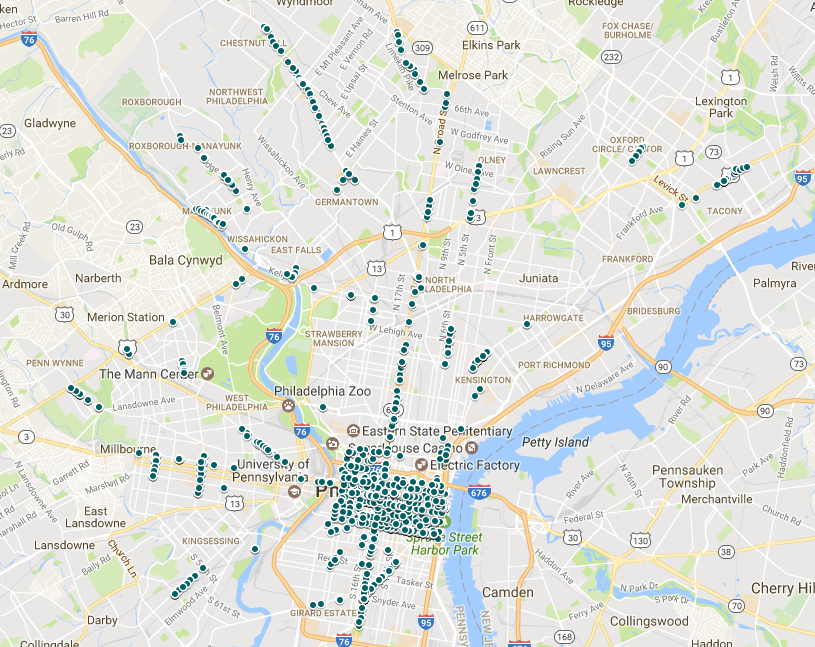
\includegraphics[width=5cm]{overview1}
		\subcaption{The whole distribution of trash bin in Philadelphia}
		\label{fig1a}}
	\qquad
	\begin{minipage}{5cm}
		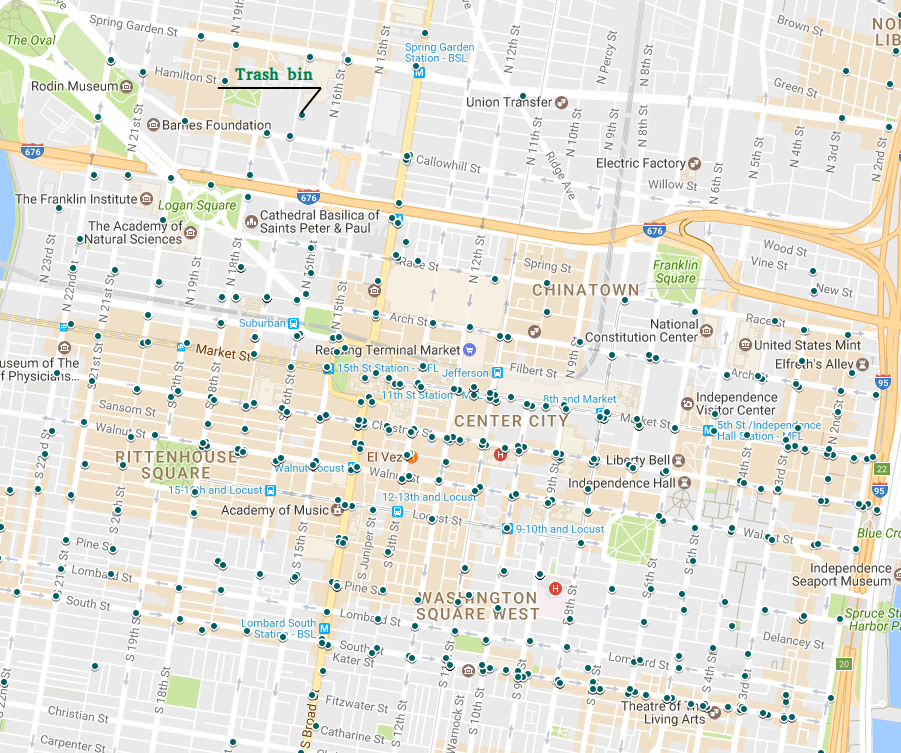
\includegraphics[width=5cm]{overview3}
		\subcaption{A part of distribution trash bin in Philadelphia}
		\label{fig1b}
	\end{minipage}
\caption{Philadelphia trash bin}
\label{Philadelphia}
\end{figure}
 
\section{IoT-Based Smart waste city management model}

\subsection{Data acquisition} 
\label{dataacquisition}
In this section, we describe how to collect waste meta data associated with their status and locations. We choose to evaluate our model with real big data in order to validate its output.
\par To obtain a set of waste data, we use an open source database, \footnote{https://www.opendataphilly.org/dataset} which has a significant amount of geo-location information and status of each bin at the largest city in the Commonwealth of Pennsylvania in the United Stated named Philadelphia. Figure \ref{Philadelphia} illustrates the distribution of trash bin (green node) in a part of Philadelphia City. We removed the content that was automatically created by stream type service. For data analysis, we adopt the following five essential fields from this meta data:
\begin{itemize}
	\item \textit{sn}: Serial number of each bin
	\item \textit{timestamp}: Milestone of recording data
	\item \textit{level}: The amount of waset in each bin at the given timestamp
	\item \textit{lat}: The latitude of each bin
	\item \textit{lon} The longitude of each bin
\end{itemize}

\par We observed that the original system has three levels of bin such as RED, YELLOW, and GREEN. So we tend to assume that the levels of bin should be HIGH, MEDIUM, and LOW, respectively. 



\subsection{System description}
\label{systemdesciption}
\subsubsection{The overview of functionality}



The proposed system is based on the waste status of each trash bin in the city. The data collected by sensors is sent over the Internet to the server where it is stored and processed. The collected data is used for monitoring and predicting the status of each bin daily. After that, they will be utilized for calculating the optimal garbage truck routes accordingly. Every day, the system sends the newly calculated routes to the workers based on the waste status, traffic congestion, the state of the forecast, and the balanced cost-efficiency functions. Since the limitation of our data, our optimal garbage truck routes is constructed based on the waste status of each bin.  The prediction status of bin can be analyzed based on the given training data before it occurs. The system overview is shown in the Figure \ref{fig2}.


\begin{figure}
	\centering
	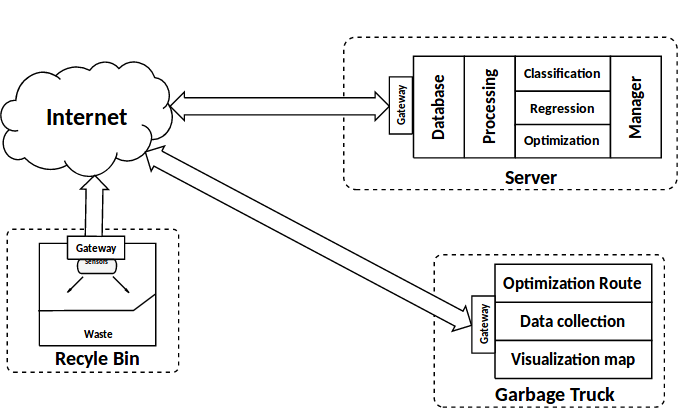
\includegraphics[width=8cm]{Model1-2}
	\caption{The smart waste management system overview}
	\label{fig2}
\end{figure}




\subsubsection{Data processing and classifications}
The status of each bin is generally not homogeneous and significantly differs from each other according to the sate of each location. In this section, we introduce an algorithm that can be used to dynamically and efficiently manage waste collection strategies.
\par K-means \cite{Kanungo2003} is an unsupervised machine learning algorithm that groups a dataset into a user-specified number (k) of clusters. We use it to make the working cluster of each garbage truck. However, this algorithm is somewhat naive, it clusters the data into k clusters, even if k is not the right number of clusters to use. Therefore, when using k-means clustering, users need some way to determine whether they are using the right number of clusters. In this paper, we use Elbow method \cite{Kodinariya2013} to validate the number of clusters. The collecting routes are the travelling cycles containing a given set of trash bins. The optimization of these cycles is a combinatorial optimization problem. When the objective function of this optimization is to minimize the driving distance. By considering the large number of routes, we use Genetic algorithm (GA) \cite{Gutierrez2008} which are relatively fast in providing near optimal solutions. Since the garbage truck needs time to collect every trash bin, it is very delightful if a status of trash bin can be predicted. Hence, after predicting, the system will recommend which one should be collected to prevent the overload case. In this paper, we use the Linear regression algorithm (LR) \cite{Ferraro2010} to predict the status of each trash bin based on the historical data with a certain confident.

\par  The overall procedure is summarized in Algorithm \ref{algorithm1}. In this algorithm, the parameters are defined in Table \ref{table1}. We suppose that the input dataset $\mathcal{D}$ is the database in \ref{dataacquisition}. The parameter $\eta$, $n$, and $k$ denotes the threshold of amount waste in each bin, the number of bins, and the number of working clusters, respectively.

\begin{table}[]
	\centering
	\caption{The definition of each variable}
	\label{table1}
	\begin{tabular}{|l|l|}
		\hline
		\centering

 Variable & Description \\ \hline
	$W=\{w_i | i \in (1,n)\}$	& The weight of each bin             \\ \hline
		$T=\{t_{di} | d \in (1,m); i \in (1,n) \}$	& \begin{tabular}[c]{@{}l@{}}The collected data milestone \\of each bin      \end{tabular}       \\ \hline
	$\mathcal{D}=\{S,L,W, T\}$	& The input data         \\ \hline
	
	$\eta$	& \begin{tabular}[c]{@{}l@{}}The threshold of amount waste \\in a bin  \end{tabular}        \\ \hline
	
	
	$\mathcal{M}=\{M_j | j \in (1,k)\}$	& 
	
	\begin{tabular}[c]{@{}l@{}}The optimal route of each \\garbage truck within each cluster\end{tabular}
  \\ \hline
  \begin{tabular}[c]{@{}l@{}}
  $\mathcal{DC}=\{DC_j | j \in (1,k)$; \\$DC_j = \{S_j, L_j, W_j, T_j\} \}$	\end{tabular}& 
  
  \begin{tabular}[c]{@{}l@{}}The working cluster\end{tabular}
  \\ \hline

  
	\end{tabular}

\end{table}


\begin{algorithm}
	\caption{Algorithm of smart waste management system }
	\begin{algorithmic}[1]
		\renewcommand{\algorithmicrequire}{\textbf{Input:}}
		\renewcommand{\algorithmicensure}{\textbf{Output:}}
		\REQUIRE $\mathcal{D}, \eta$
		\ENSURE  $\mathcal{M}$
		\\ \textit{Initialization}: 
		\STATE $k$ = Elbow ($\mathcal{D}\rightarrow$L)
		\STATE $\mathcal{DC}$ = Kmeans ($\mathcal{D}\rightarrow$L, $k$)
		\FOR {$j = 1$ to $k$}
		\FOR {$h = 1$ to size($DC_j$)}
		\IF {($s_{jh} \ge \eta$)}
		\STATE $w_{jh} = 1$
		\STATE $M_j$ = Optimalroute ($DC_j \rightarrow L_j, DC_j \rightarrow W_j$)
		
		\ENDIF
		\ENDFOR
		\ENDFOR
		
		\RETURN $\mathcal{M}$ 
	\end{algorithmic} 
\label{algorithm1}
\end{algorithm}

% An example of a floating figure using the graphicx package.
% Note that \label must occur AFTER (or within) \caption.
% For figures, \caption should occur after the \includegraphics.
% Note that IEEEtran v1.7 and later has special internal code that
% is designed to preserve the operation of \label within \caption
% even when the captionsoff option is in effect. However, because
% of issues like this, it may be the safest practice to put all your
% \label just after \caption rather than within \caption{}.
%
% Reminder: the "draftcls" or "draftclsnofoot", not "draft", class
% option should be used if it is desired that the figures are to be
% displayed while in draft mode.
%
%\begin{figure}[!t]
%\centering
%\includegraphics[width=2.5in]{myfigure}
% where an .eps filename suffix will be assumed under latex, 
% and a .pdf suffix will be assumed for pdflatex; or what has been declared
% via \DeclareGraphicsExtensions.
%\caption{Simulation results for the network.}
%\label{fig_sim}
%\end{figure}
 
% Note that the IEEE typically puts floats only at the top, even when this
% results in a large percentage of a column being occupied by floats.
 
 
% An example of a double column floating figure using two subfigures.
% (The subfig.sty package must be loaded for this to work.)
% The subfigure \label commands are set within each subfloat command,
% and the \label for the overall figure must come after \caption.
% \hfil is used as a separator to get equal spacing.
% Watch out that the combined width of all the subfigures on a 
% line do not exceed the text width or a line break will occur.
%
%\begin{figure*}[!t]
%\centering
%\subfloat[Case I]{\includegraphics[width=2.5in]{box}%
%\label{fig_first_case}}
%\hfil
%\subfloat[Case II]{\includegraphics[width=2.5in]{box}%
%\label{fig_second_case}}
%\caption{Simulation results for the network.}
%\label{fig_sim}
%\end{figure*}
%
% Note that often IEEE papers with subfigures do not employ subfigure
% captions (using the optional argument to \subfloat[]), but instead will
% reference/describe all of them (a), (b), etc., within the main caption.
% Be aware that for subfig.sty to generate the (a), (b), etc., subfigure
% labels, the optional argument to \subfloat must be present. If a
% subcaption is not desired, just leave its contents blank,
% e.g., \subfloat[].
 
 
% An example of a floating table. Note that, for IEEE style tables, the
% \caption command should come BEFORE the table and, given that table
% captions serve much like titles, are usually capitalized except for words
% such as a, an, and, as, at, but, by, for, in, nor, of, on, or, the, to
% and up, which are usually not capitalized unless they are the first or
% last word of the caption. Table text will default to \footnotesize as
% the IEEE normally uses this smaller font for tables.
% The \label must come after \caption as always.
%
%\begin{table}[!t]
%% increase table row spacing, adjust to taste
%\renewcommand{\arraystretch}{1.3}
% if using array.sty, it might be a good idea to tweak the value of
% \extrarowheight as needed to properly center the text within the cells
%\caption{An Example of a Table}
%\label{table_example}
%\centering
%% Some packages, such as MDW tools, offer better commands for making tables
%% than the plain LaTeX2e tabular which is used here.
%\begin{tabular}{|c||c|}
%\hline
%One & Two\\
%\hline
%Three & Four\\
%\hline
%\end{tabular}
%\end{table}
 
 
% Note that the IEEE does not put floats in the very first column
% - or typically anywhere on the first page for that matter. Also,
% in-text middle ("here") positioning is typically not used, but it
% is allowed and encouraged for Computer Society conferences (but
% not Computer Society journals). Most IEEE journals/conferences use
% top floats exclusively. 
% Note that, LaTeX2e, unlike IEEE journals/conferences, places
% footnotes above bottom floats. This can be corrected via the
% \fnbelowfloat command of the stfloats package.
 
 
 
 
\section{Conclusion}
The conclusion goes here.
 
 
 
 
% conference papers do not normally have an appendix
 
 
 
% use section* for acknowledgment
\ifCLASSOPTIONcompsoc
  % The Computer Society usually uses the plural form
  \section*{Acknowledgments}
\else
  % regular IEEE prefers the singular form
  \section*{Acknowledgment}
\fi
 
 
The authors would like to thank...
 
 
 
 
 
% trigger a \newpage just before the given reference
% number - used to balance the columns on the last page
% adjust value as needed - may need to be readjusted if
% the document is modified later
%\IEEEtriggeratref{8}
% The "triggered" command can be changed if desired:
%\IEEEtriggercmd{\enlargethispage{-5in}}
 
% references section
 
% can use a bibliography generated by BibTeX as a .bbl file
% BibTeX documentation can be easily obtained at:
% http://mirror.ctan.org/biblio/bibtex/contrib/doc/
% The IEEEtran BibTeX style support page is at:
% http://www.michaelshell.org/tex/ieeetran/bibtex/
%\bibliographystyle{IEEEtran}
% argument is your BibTeX string definitions and bibliography database(s)
%\bibliography{IEEEabrv,../bib/paper}
%
% <OR> manually copy in the resultant .bbl file
% set second argument of \begin to the number of references
% (used to reserve space for the reference number labels box)
\begin{thebibliography}{1}
\bibitem{Delicato2013}
F. C. Delicato, P. F. Pires,  T. Batista, E. Cavalcante, B. Costa, and  T. Barros, \emph{Towards an IoT eco-system}, In the Proceedings of the 1st ACM International Workshop on Software Engineering for Systems-of-Systems, SESoS’13, 2013, pp. 25--28.


\bibitem{Lazarescu2013}
M. T. Lazarescu, \emph{Design of a WSN platform for long-term environmental monitoring for IoT application}, IEEE Journal on Emerging and Selected Topics in Circuits and Systems, Volume 3, Number 1 (2013): 45--54.



\bibitem{Kelly2013}
S. D. T. Kelly, N. K. Suryadevara, and S. C. Mukhopadhyay, \emph{Towards the implementation of IoT for environmental condition monitoring in homes}, IEEE Sensors Journal, Volume 13, Number 10 (2013): 3846--3853.

\bibitem{Gama2012}
K. Gama, L. Touseau, and D. Donsez, \emph{Combining heterogeneous service technologies for building an internet of things middle-ware}, Computer Communications, Volume 35, Number 4 (2012): 405--417.


\bibitem{Foschini2011}
L. Foschini, T, Taleb, A. Corradi, and D. Bottazzi, \emph{M2M-based metropolitan platform for IMS-enabled road traffic management in IoT}, IEEE Communications Magazine, Volume 49, Number 11 (2011): 50--57.


\bibitem{Jara2011}
A. J. Jara, A. Zamora, and A. F. G. Skarmeta, \emph{An internet of things-based personal device for diabetes therapy management in ambient assited living (AAL)}, Personal and Ubiquitous Computing, Volume 15, Number 4 (2011): 431--440.




\bibitem{Tozlu2012}
S. Tozlu, M. Senel, W. Mao, and A. Keshavarzian, \emph{Wi-Fi enabled sensors for internet of things: A pratical approach}, IEEE Communications Magazine, Volume 50, Number 6 (2012): 134--143.

\bibitem{Li2011}
X. Li, R. Lu, X. Liang, X. Shen, J. Chen, and X. Lin, \emph{Smart community: An internet of things appilication}, IEEE Communications Magazine, Volume 49, Number 11 (2011): 68--75.

\bibitem{Medvedev2015}
A. Medvedev, P. Fedchenkov, A. Zaslavsky, T. Anagnostopoulos, and S. Khoruzhnikov, \emph{Waste management as an IoT enabled service in smart cites}, 15th ed, St. Petersburg, Russia: Internet of Things, Smart Spaces, and Next Generation Networks and Systems, 2015, pp 104--115.



\bibitem{Gutierreza2015}
J. M. Gutierreza, M. Jensenb, M. Heniusa, and T. Riaze, \emph{Smart waste collection system based on location intelligence}, Procedia Computer Science 61 (2015): 120--127.


\bibitem{Hong2014}
J. Hong, S. Park, B. Lee, J. Lee, D. Jeong, and S. Park, \emph{IoT-based smart garbage system for efficient food waste management}, The Scientific World Journal (2014).




\bibitem{Buhrkala212}
K. Buhrkala, A. Larsena, and S. Ropkea, \emph{The waste collection vehicle routing problem with time windows in a city logistics context}, Procedia Social and Behavioral Sciences 39 (2012): 241--254.


\bibitem{Nuorito2006}
T. Nuortio, J. Kyt\"ojoki, H. Niska, and O. Br\"aysy, \emph{Improved route planning and scheduling of waste collection and transport}, Expert Systems with Applications, Volume 30, Issue 2 (2006): 223--232.


\bibitem{Sharma2015}
N. Sharma, N. Singha, and T. Dutta, \emph{Smart bin implementation for smart cities}, International Journal of Scientific \& Engineering Research (2015), Volume 6, Issue 9: 787--791.


\bibitem{Glouche2013}
Y. Glouche and P. Couderc, \emph{A smart waste management with self-describing objects}, The second International Conference on Smart Systems, Devices, and Technologies, 2013, pp 63--70.


\bibitem{Sinhan2013}
A. Sinhan and P. Couderc, \emph{Smart bin for imcompatible waste items}, The ninth International Conference on Autonomic and Autonomous Systems, 2013, pp 40--45.


\bibitem{Kanungo2003}
 T. Kanungo, D.M. Mount, N.S. Netanyahu, C.D. Piatko, R. Silverman, and A.Y. Wu, \emph{An efficient k-means clustering algorithm: Analysis and implementation}, IEEE Transactions on Pattern Analysis and Machine Intelligence, Volume 24, Issue 7 (2002): 881--892.


\bibitem{Kodinariya2013}
T. M. Kodinariya and P. R. Makwana, \emph{Review on determining number of cluster in K-means clustering}, International Journal of Advance Research in
Computer Science and Management Studies, Volume 1, Issue 6 (2013): 90--95.


\bibitem{Gutierrez2008}
J. M. Gutierrez, M. Imine, and O. B. Madsen, \emph{Network planning using GA for regular topologies}, Proceedings of IEEE International Conference on Communications, 2008, pp: 5258--5262.


\bibitem{Ferraro2010}
M. B. Ferraro, R. Coppi, G. Gonz\'alez, Rodr\'iguez, and A. Colubi, \emph{A linear regression model for imprecise response}, International Journal of Approximate Reasoning Volume 51, Number 7 (2010): 759--770.







\end{thebibliography}
 
 
 
 
% that's all folks
\end{document}
 
 
 
